\subsection{Simulation von Argon}
\subsubsection{Gasförmiges Argon}
Der Temperaturverlauf des Argons für verschiedene Zeiträume der Abkühlung ist in Abb. \ref{fig:cool_temp1ns}) bis \ref{fig:cool_temp10ns}) dargestellt.
Die dazugehörige potentielle Energie ist in Abb. \ref{fig:cool_pot1ns}) bis \ref{fig:cool_pot10ns}) zu sehen.
\begin{figure}
  \centering
  \vspace{-0.3cm}
  \begin{subfigure}[h]{0.45\textwidth}
    \centering
    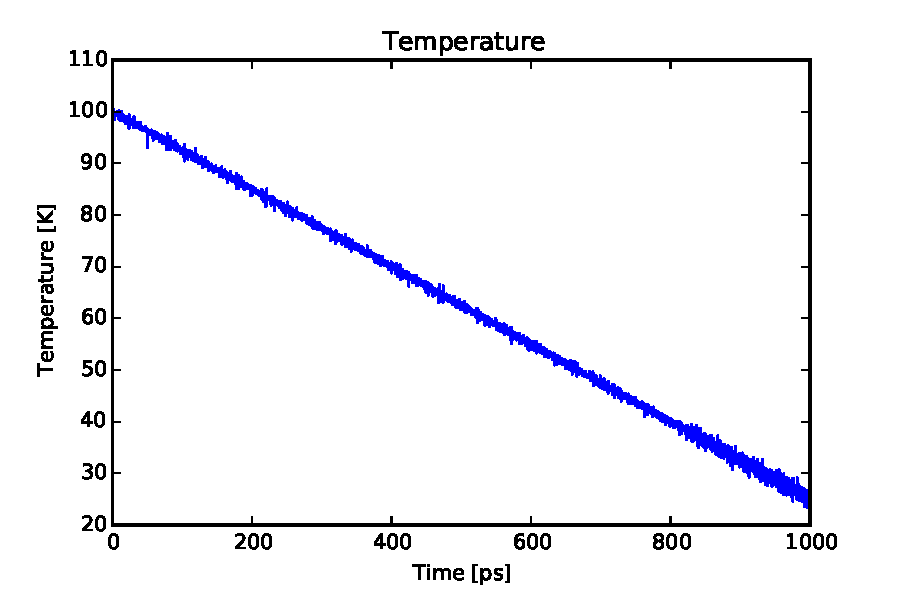
\includegraphics[width=\textwidth]{/home/winz3r/Documents/Protokolle/moleculardynamic/temp_cool__1n.pdf}
    \caption{\centering Temperaturverlauf für das Abkühlen in 1~ns.}\label{fig:cool_temp1ns}
  \end{subfigure}
  \vspace{0.25cm}
  \centering
  \begin{subfigure}[h]{0.45\textwidth}
    \centering
    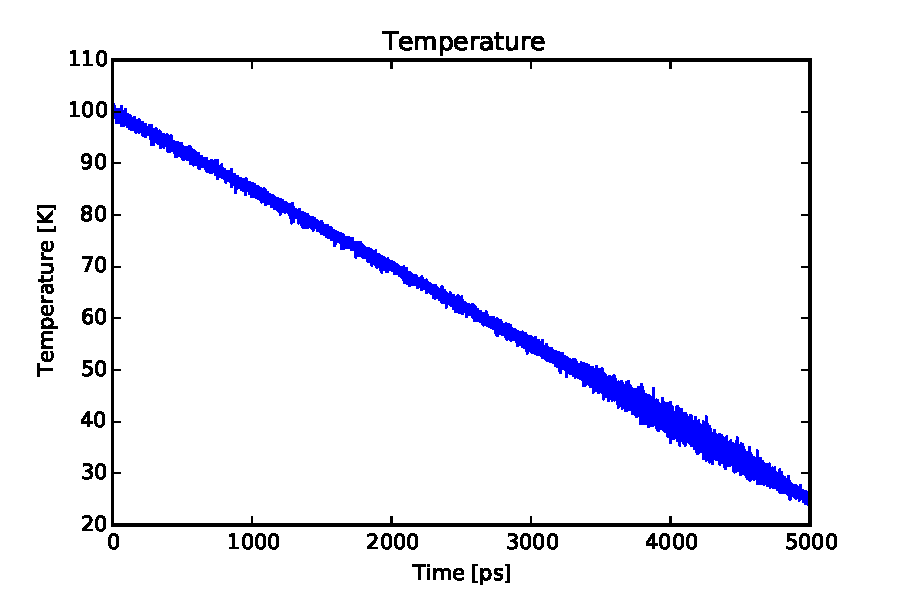
\includegraphics[width=\textwidth]{/home/winz3r/Documents/Protokolle/moleculardynamic/temp_cool__5n.pdf}
    \caption{\centering Temperaturverlauf für das Abkühlen in 5~ns.}\label{fig:cool_temp5ns}
  \end{subfigure}
  \vspace{0.25cm}
  \centering
  \begin{subfigure}{\textwidth}
    \centering
    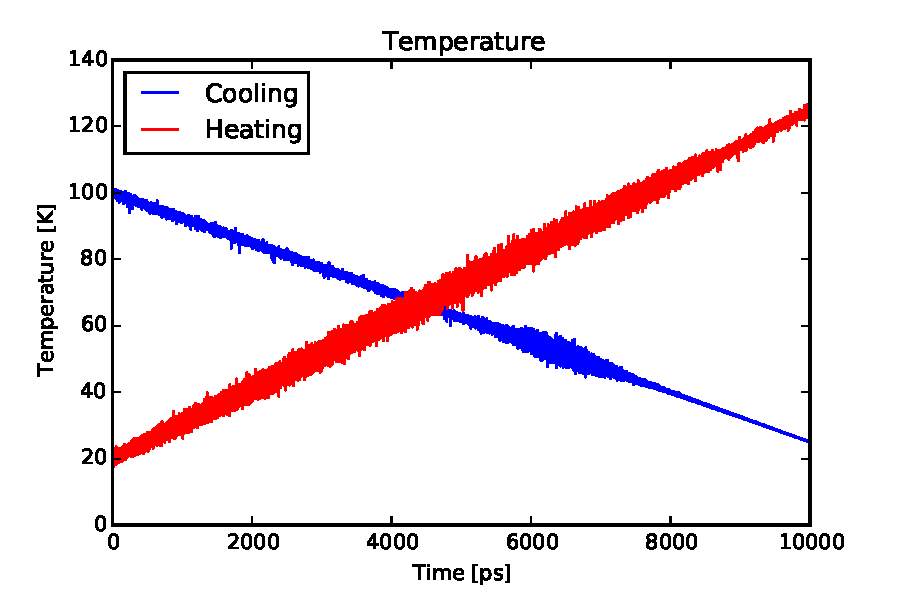
\includegraphics[width=0.65\textwidth]{/home/winz3r/Documents/Protokolle/moleculardynamic/heatup_temp.pdf}
    \caption{Temperaturverlauf für das Abkühlen und Erwärmen in 10~ns.}\label{fig:cool_temp10ns}
  \end{subfigure}
  \caption{Temperaturverläufe der Simulationen von gasförmigen Argon beim Abkühlen bzw. Erwärmen.}
\end{figure}
\begin{figure}
  \centering
  \vspace{-0.3cm}
  \begin{subfigure}[h]{0.45\textwidth}
    \centering
    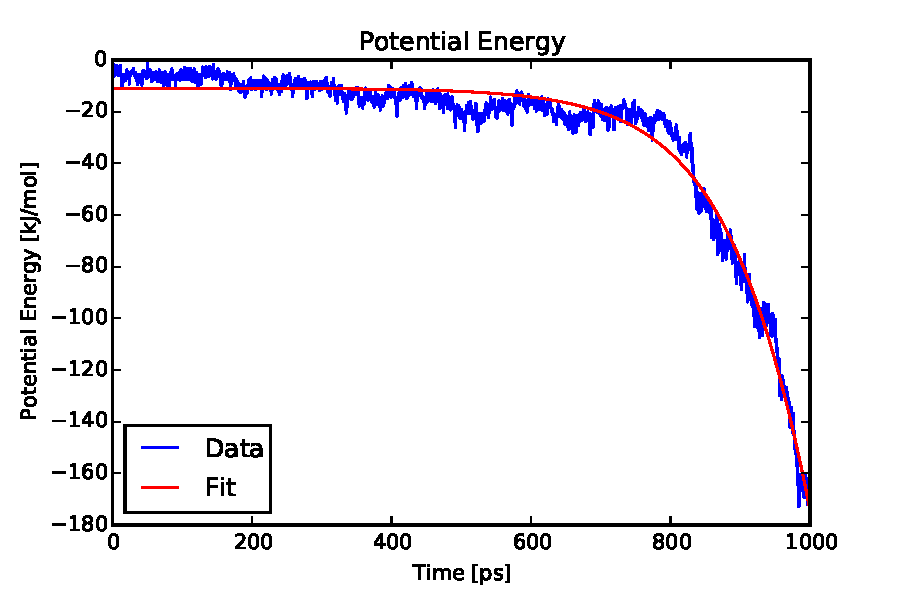
\includegraphics[width=\textwidth]{/home/winz3r/Documents/Protokolle/moleculardynamic/pot_cool__1n.pdf}
    \caption{\centering Verlauf der potentiellen Energie für das Abkühlen in 1~ns.}\label{fig:cool_pot1ns}
  \end{subfigure}
  \vspace{0.25cm}
  \centering
  \begin{subfigure}[h]{0.45\textwidth}
    \centering
    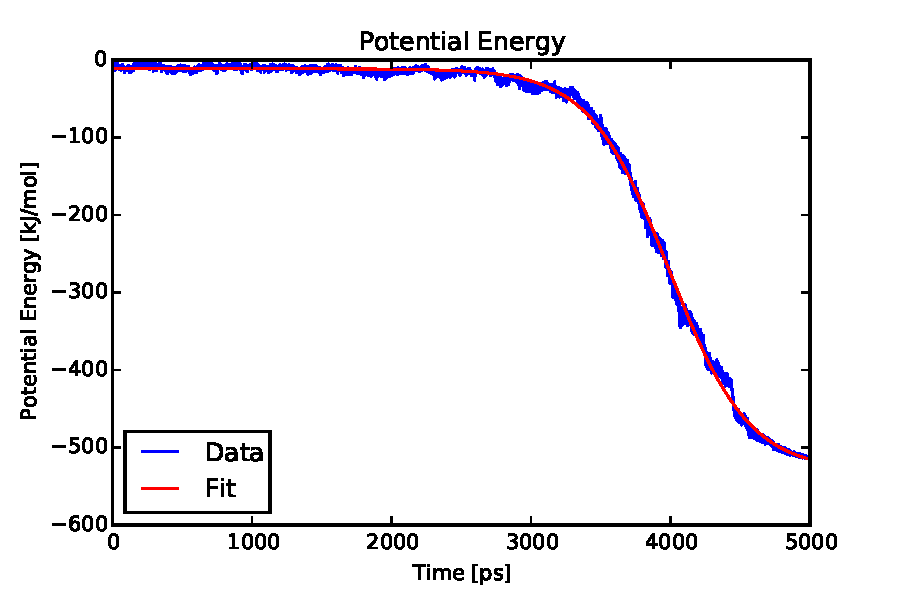
\includegraphics[width=\textwidth]{/home/winz3r/Documents/Protokolle/moleculardynamic/pot_cool__5n.pdf}
    \caption{\centering Verlauf der potentiellen Energie für das Abkühlen in 5~ns.}\label{fig:cool_pot5ns}
  \end{subfigure}
  \vspace{0.25cm}
  \centering
  \begin{subfigure}{\textwidth}
    \centering
    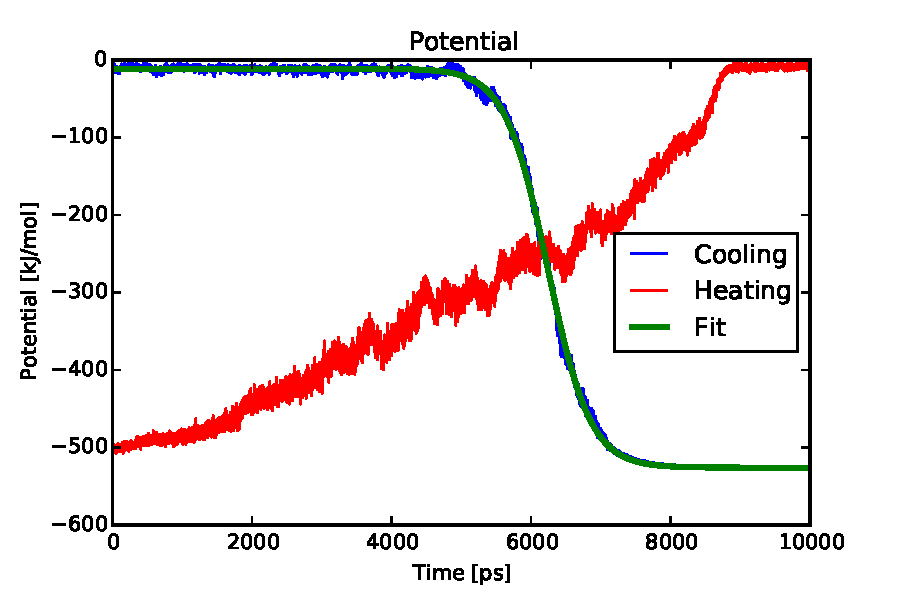
\includegraphics[width=0.65\textwidth]{/home/winz3r/Documents/Protokolle/moleculardynamic/heatup_pot.pdf}
    \caption{Verlauf der potentiellen Energie für das Abkühlen und Erwärmen in 10~ns.}\label{fig:cool_pot10ns}
  \end{subfigure}
  \caption{Potentielle Energie der Simulationen von gasförmigen Argon beim Abkühlen bzw. Erwärmen.}
\end{figure}
Zusätzlich ist in den Abbildungen \ref{fig:cool_temp10ns}) und \ref{fig:cool_pot10ns}) der Vergleich zwischen Erwärmen und Abkühlen des Argon Gases zu sehen.

\\ \noindent
Aus dem Verlauf der potentiellen Energie lässt sich der Siedepunkt des Argongases bestimmen. Dazu wird eine Logistische Kurve,
\begin{align}
f(x)=\frac{L}{1+\exp\left[ -k \left(x-x_0\right)\right]} + y_0
\end{align}
an die Messwerte gefitted.
Zum Fitten wird eine \emph{python-scipy} Funktion benutzt, die Gebrauch von dem \emph{Levenberg–Marquardt} Algorithmus macht \cite{leastsquares}.
\\ \noindent
Das Maximum der Ableitung der Kurve entspricht dem Siedepunkt. Es liegt bei $x = x_0$.
Der Siedepunkt konnte aus den drei verschiedenen Abkühlvorgängen bestimmt werden, die Ergebnisse sind in Tabelle \ref{tab:siedepunkt}) aufgeführt.

\begin{table}
\centering
\caption{Siedepunkte wie sie aus den verschiedenen Simulationen bestimmt wurden. Zur Bestimmung der Temperatur wurde ein linearer Zusammenhang zwischen Temperatur und Zeit angenommen der aus dem Versuchsaufbau und Abb. \ref{fig:cool_temp1ns}) bis \ref{fig:cool_temp10ns}) hervorgeht.}\label{tab:siedepunkt}
\begin{tabular}{l|rrr}
Abkühlzeit [ns] & $x_0$ [ps] & Temperatur [K] \\ \hline
1 & 1150(20) &  14(2) \\
5 & 3990(1) & 40.15(1) \\
10 & 6239.6(2) & 53.203(2) \\
\end{tabular}
\end{table}

Der Siedepunkt von Argon ist stark vom Druck abhängig. Der Druck in dem simulierten System lässt sich unter Verwendung der van-der-Waals Gleichung bestimmen. Die Simulationsbox hat eine Kantenlänge von 7.7395~nm mit 100 Argon Atomen in der Box.
Dies ergibt mit Werten für $a = 1.355~$L$^2$bar/mol$^2$ und $b=0.03201$~L/mol \cite{chemicalcrc} einen Druck von ca. 2.8~bar bei 100~K.
\\ \noindent
Bei diesem Druck hat Argon einen Siedepunkt von ca. 98~K \cite{phasediagram}. Bei einem atmosphärischem Druck von 1~bar liegt der Siedepunkt bei 87~K.


%Kondensation von Argon
% Energieplots Temperaturplot verschiedene Abkühlzeiten auf Differenzen der Siedepunkte achten.
%
\subsubsection{Flüssiges Argon}
%
%Druck 216 Atome=5.8~Bar
% siedepunkt = 107~K
Als nächstes wird das Gefrieren von flüssigem Argon betrachtet. Der Druck des Gases bei 100~K entspricht etwa 5.8~bar, der Siedepunkt bei diesem Druck liegt bei ca. 107~K \cite{phasediagram}.
In Abb. \ref{fig:liqtemp}) und \ref{fig:liqpot} ist der Verlauf der Temperatur und der potentiellen Energie zu sehen.
Das Gefrieren des Argons setzt bei einer Temperatur von ca. 45~K ein. 
\begin{figure}
\begin{subfigure}{0.45\textwidth}\centering
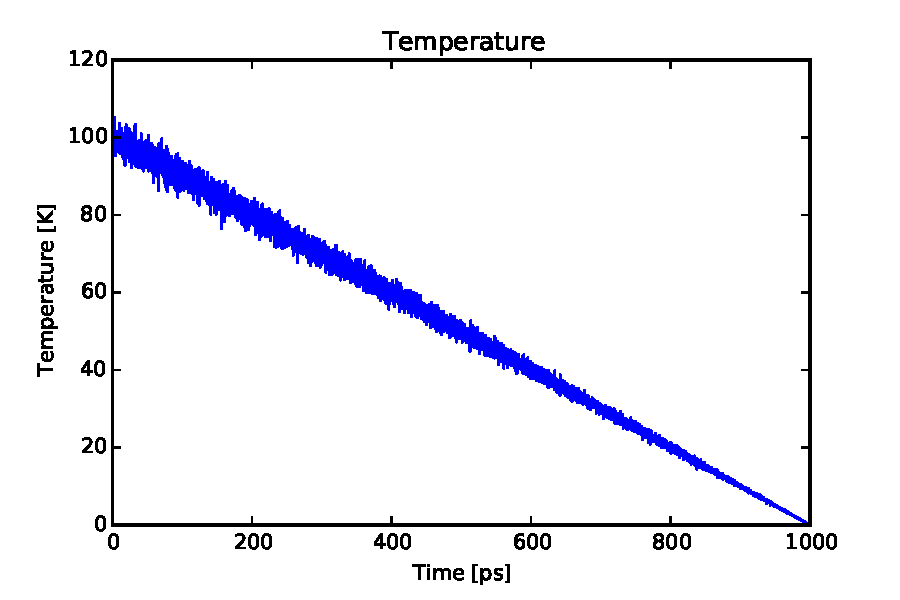
\includegraphics[width=\textwidth]{/home/winz3r/Documents/Protokolle/moleculardynamic/temp_cool_ui.pdf}\caption{\centering Verlauf der Temperatur beim Abkühlen von flüssigem Argon von 100~K auf 25~K, bei einem Druck von 5.8~bar.}\label{fig:liqtemp}
\end{subfigure}
\hspace{0.5cm}
\begin{subfigure}{0.45\textwidth}\centering
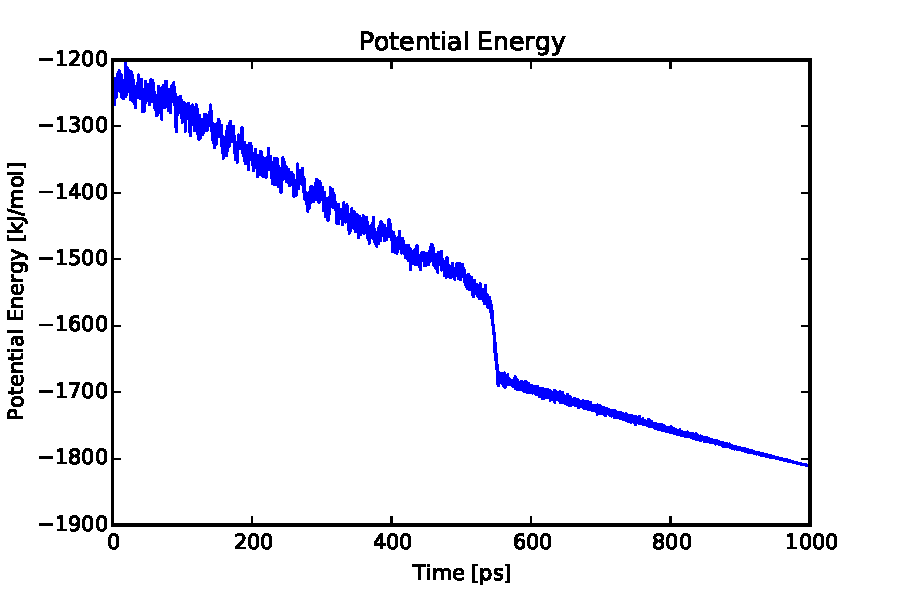
\includegraphics[width=\textwidth]{/home/winz3r/Documents/Protokolle/moleculardynamic/pot_cool_qui.pdf}\caption{\centering Verlauf der potentiellen Energie beim Abkühlen von flüssigem Argon von 100~K auf 25~K, bei einem Druck von 5.8~bar.}\label{fig:liqpot}
\end{subfigure}
\caption{Gefrieren von Argon.}
\end{figure}
\noindent
Es lässt sich außerdem die Anzahl der Atome in einem bestimmten Abstand eines Atoms bestimmen. Dies ist in Abb. \ref{fig:nearest}) dargestellt. Die Verteilung ist zu Beginn in der flüssigen Phase und am Ende der Simulation in der festen Phase bestimmt worden.
\begin{figure}
\centering
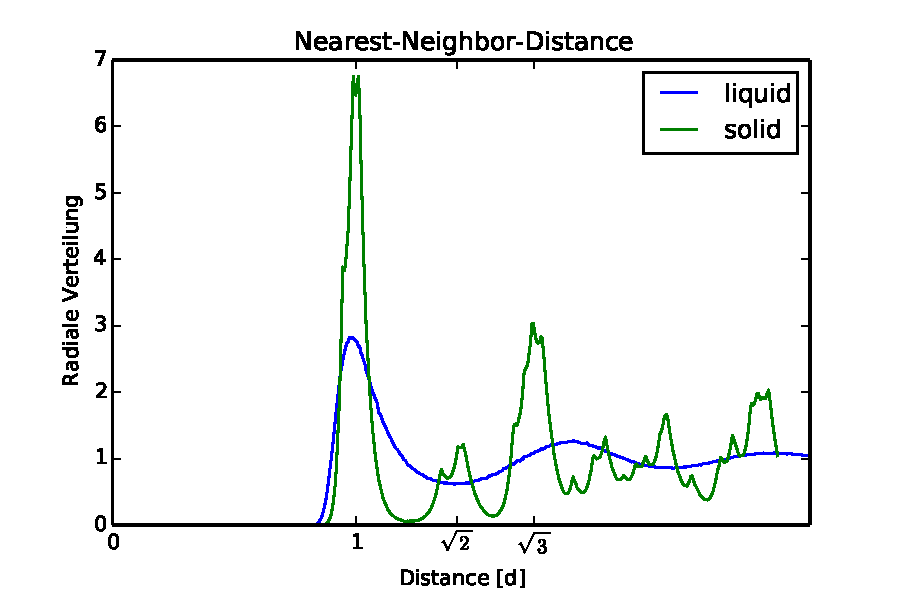
\includegraphics[width=0.75\textwidth]{/home/winz3r/Documents/Protokolle/moleculardynamic/nearest.pdf}\caption{ \centering Radiale Verteilung der Argonatome als Funktion des Abstandes von einem Atom. Der Abstand ist in Einheiten des Durchmessers eines Argonatomes dargestellt ($d=0.376$~nm). Die Verteilung wurde zu Beginn der Simulation und nach Ende der Simulation als Mittel über ein Zeitintervall festgestellt.
Das Auftreten der Peaks im Festkörper entspricht dem theroretisch erwarteten \emph{fcc}-Gitter eines Argon-Kristalls.}\label{fig:nearest}
\end{figure}
\noindent
Zudem lässt sich die Diffusionskonstante des Argons bestimmen. Dazu wird die Einstein'sche Diffusionsrelation auf die durchschnittliche quadratische Abweichung vom Startpunkt bezogen. \emph{GROMACS} liefert hierfür ein Ergebnis von $2.5(1)\cdot 10 ^{-5}$~cm$^2$/s, der experimentelle Wert liegt bei $2.43 \cdot
10^{-5}$~cm$^2$/s.
%Gefrieren von Argon
% Diffusionskonstante
% Radialplot
% Gefrierpunkt
\subsection{Simulation von Proteinen}
\subsubsection{Protein G B1}
Eine mit \emph{VMD} erzeugte 3d-Darstellung der B1 Domäne des Proteins G ist in Abb. \ref{fig:3dpgb}) zu sehen.
die gelben Pfeile stellen $\beta$-Faltblatt Strukturen da, und die violette Spirale eine $\alpha$-Helix Struktur. In grau sind Verbindungen zwischen den Sekundärstrukturen dargestellt.
\begin{figure}
\centering
\includegraphics[width=0.5\textwidth]{/home/winz3r/Desktop/philip_vitali-06012016/protein/path3367.png}\caption{Dreidimensionale Darstellung der B1 Domäne des Proteins G. Gelb: $\beta$-Faltblatt; Violett: $\alpha$-Helix.}\label{fig:3dpgb}
\end{figure}
\noindent
Wie stark die durchschnittlichen Positionen der Atome des Proteins von ihrer Anfangsposition abweichen, ist in Abb. \ref{fig:rmsd}) als Funktion der Zeit aufgetragen. Der starke Anstieg zu Beginn der Simulation wird durch Minimierung der freien Energie verursacht.
Im Gegensatz zur Minimierung der Energie wird nun nicht mehr nur die potentielle Energie minimiert.
Das Verhalten der potentiellen Energie wird in Abb. \ref{fig:rmpot}) veranschaulicht.
Die Fluktuationen der einzelnen Aminosäuren ist in Abb. \ref{fig:rmsf} dargestellt. Zu erkennen sind deutliche Fluktuationen an den Residuen
1, 11, 14, 21, 24 und 42.
\\ \noindent
Die mit dem Lösungsmittel in Kontakt stehende Oberfläche des Proteins, lässt sich Abb. \ref{fig:rmsurf}) entnehmen. Der hohe Anteil an hydrophober Oberfläche hängt mit der Funktion des Proteins als Membranprotein zusammen. Die Tatsache, dass sowohl die hydrophile als auch die hydrophobe Oberfläche nur schwach fluktuieren bedeutet, dass sich das Protein nicht stark faltet.
\\ \noindent
Die durchschnittliche Ausdehnung des Proteins, der Gyrationsradius ist in Abb. \ref{fig:rmgyr}) dargestellt.
\\ \noindent
Das Verhalten der Sekundärstrukturen des Proteins G B1 wird in Abb. \ref{fig:sekund}) als Funktion der Zeit farbkodiert aufgetragen. Man kann erkennen, dass die Sekundärstrukturen
größtenteils stabil sind und nur an ihren Grenzen schwach fluktuieren.
\begin{figure}
\begin{subfigure}{0.45\textwidth}
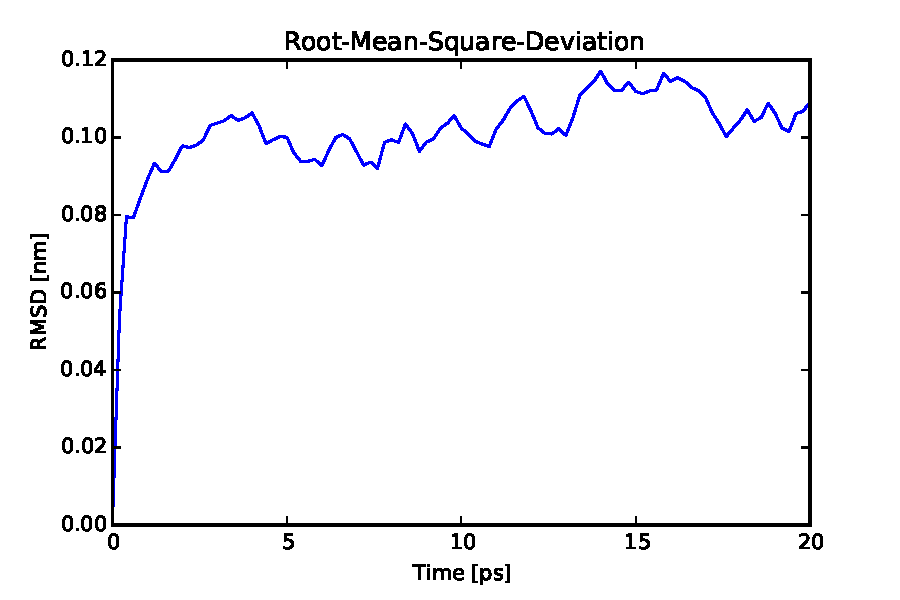
\includegraphics[width=\textwidth]{/home/winz3r/Documents/Protokolle/moleculardynamic/rmsd.pdf}\caption{\centering Durchschnittliche Abweichung der Atompositionen als Funktion der Zeit.}\label{fig:rmsd}
\end{subfigure}
\hspace{0.1cm}
\begin{subfigure}{0.45\textwidth}
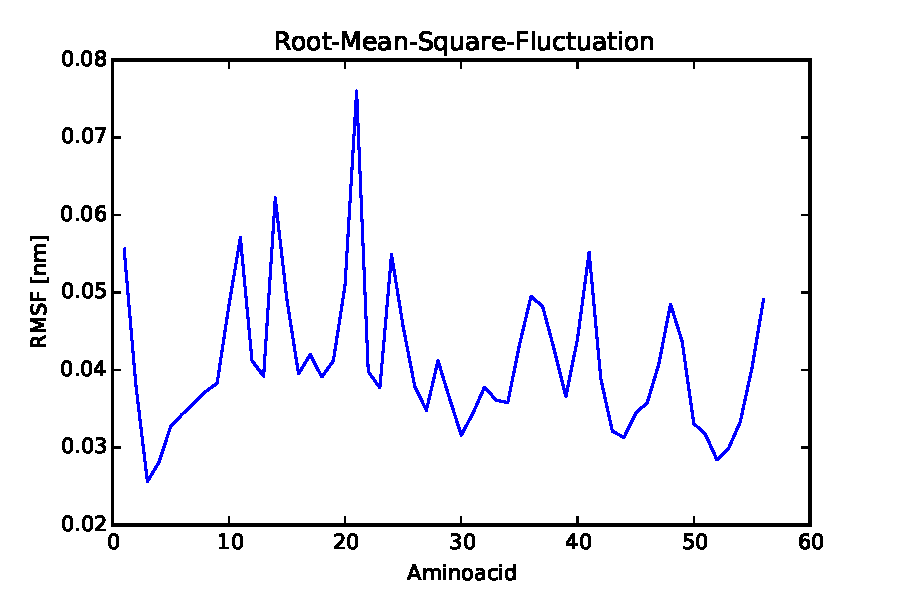
\includegraphics[width=\textwidth]{/home/winz3r/Documents/Protokolle/moleculardynamic/rmsf.pdf}\caption{\centering Durchschnittliche Fluktuationen der einzelnen Aminosäuren.}\label{fig:rmsf}
\end{subfigure}
\vspace{0.5cm}
\begin{subfigure}{0.45\textwidth}
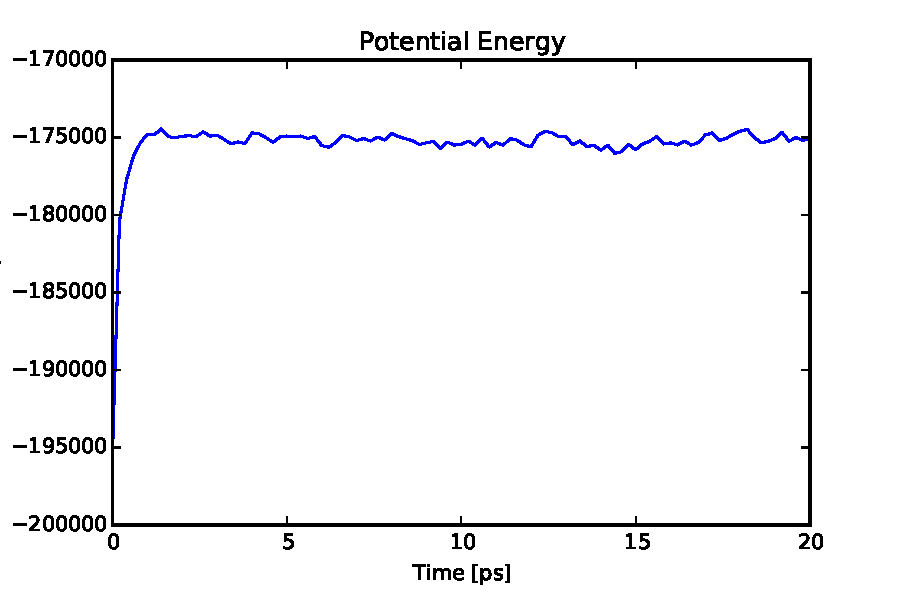
\includegraphics[width=\textwidth]{/home/winz3r/Documents/Protokolle/moleculardynamic/rmspot.pdf}\caption{\centering Anstieg der potentiellen Energie (kJ/mol) als Resultat der Minimierung der freien Energie.}\label{fig:rmspot}
\end{subfigure}
\hspace{1cm}
\begin{subfigure}{0.45\textwidth}
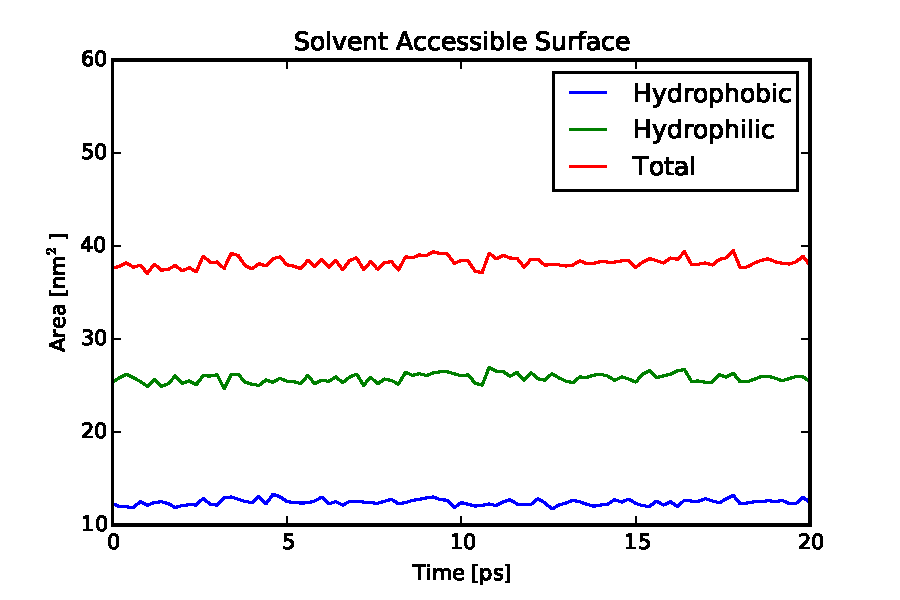
\includegraphics[width=\textwidth]{/home/winz3r/Documents/Protokolle/moleculardynamic/surface.pdf}\caption{\centering Mit der Lösung in Kontakt stehende Fläche des Proteins.}\label{fig:rmsurf}
\end{subfigure}
\vspace{0.5cm}
\begin{subfigure}{0.45\textwidth}
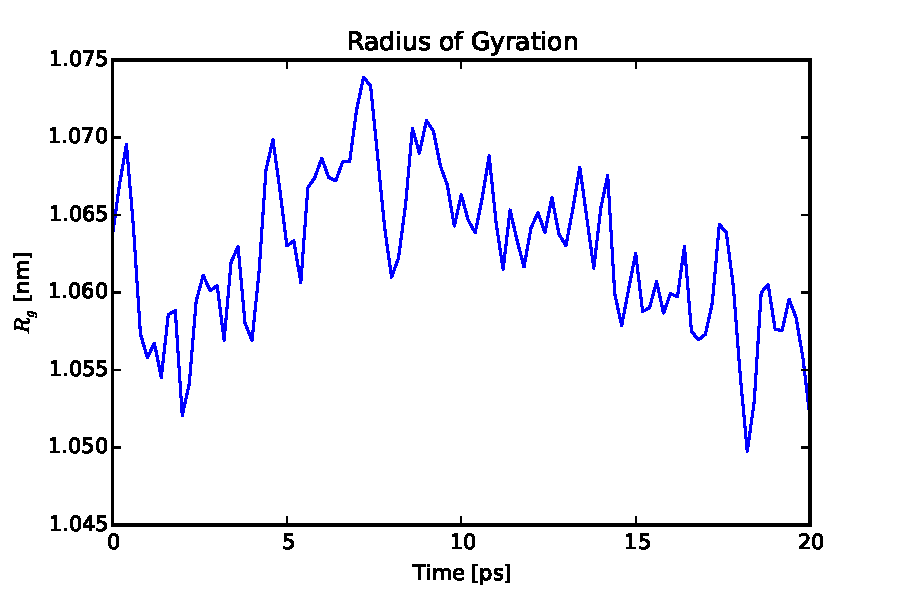
\includegraphics[width=\textwidth]{/home/winz3r/Documents/Protokolle/moleculardynamic/gyration.pdf}\caption{\centering Gyrationsradius des Proteins in Abhängigkeit von der Zeit.}\label{fig:rmgyr}
\end{subfigure}
\hspace{1cm}
\begin{subfigure}{0.45\textwidth}
\includegraphics[width=\textwidth]{/home/winz3r/Desktop/philip_vitali-06012016/protein/plot_eps.png}\caption{\centering Verhalten der Sekundärstrukturen als Funktion der Zeit.}\label{fig:sekund}
\end{subfigure}
\caption{Simulation des Proteins G B1 über einen Zeitraum von 20ps.}
\end{figure}

\subsubsection{PCA von T4-Phagen Lysozym}
Die PCA der vorbereiteten Bewegung von T4-Phagen Lysozym liefert Hauptkomponenten mit den in Abb. \ref{fig:pca_val}) aufgetragenen Varianzen. Obwohl es mehr als 480 Atome im Lysozym gibt und damit mehr als 1400 Hauptkomponenten, wird ersichtlich, dass die Bewegung nur in wenigen linear unabhängigen Richtungen stattfindet. Hauptkomponenten mit einer dazugehörigen Varianz nah bei null sind auf die starke Bindung zwischen Atomen einer Aminosäure zurückzuführen und auf Symmetrien, wie die Translationsinvarianz des Systems.
Die kumulative Varianz der ersten beiden Hauptkomponenten umfasst bereits mehr als 90\% der gesamten Varianz der Atompositionen.
\\ \noindent
In Abb. \ref{fig:pca_comp}) sieht man die Bewegung des Lysozyms entlang der ersten acht Hauptkomponenten.
Aus den Projektionen kann der Einfluss der Hauptkomponenten auf die gesamt Bewegung abgeschätzt werden. Es ist allerdings einfacher nur die Hauptkomponenten zur Visualisierung und Analyse zu verwenden, die den größten Beitrag zur Varianz der Atompositionen liefern.
Da es zum Visualisieren der Bewegung simpler ist nur zwei Dimensionen zu betrachten werden nur die ersten beiden Hauptkomponenten zur weiteren Analyse herangezogen.
\\ \noindent
In Abb. \ref{fig:move}) sind die Bewegungen entlang der ersten beiden Hauptkomponenten in der 3d-Darstellung des Lysozyms skizziert (rot: erste Hauptkomponente; blau: zweite Hauptkomponente).
\begin{figure}
\centering
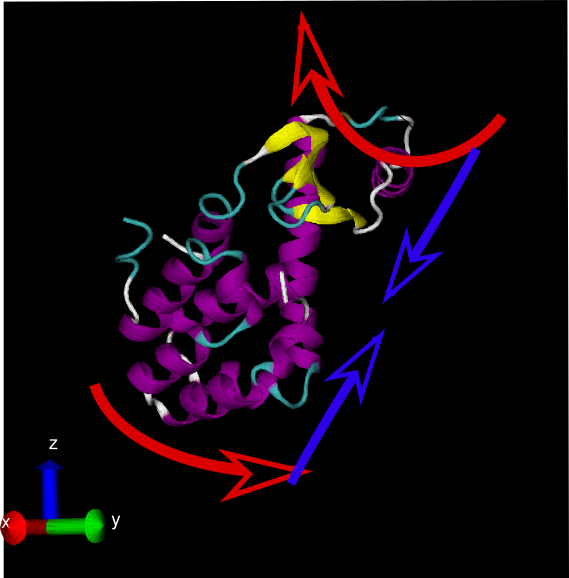
\includegraphics[width=0.6\textwidth]{/home/winz3r/Desktop/philip_vitali-06012016/pca/g3365.png}\caption{Skizze der Scher- und Klappbewegung des Lysozyms. Die erste Hauptkomponente entspricht der Scherbewegung (rot), die zweite einer Klappbewegung (blau).}\label{fig:move}
\end{figure}

\begin{figure}
\centering
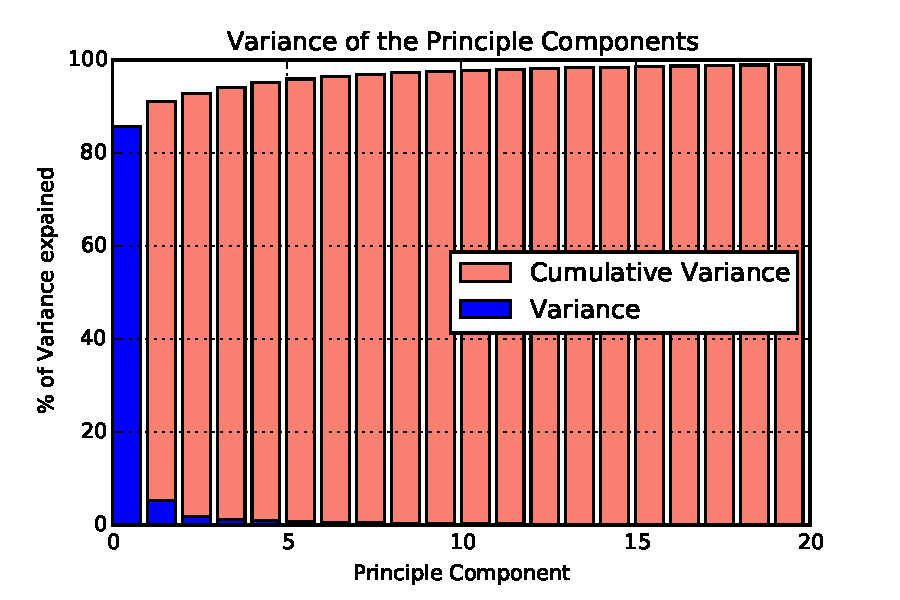
\includegraphics[width=0.7\textwidth]{/home/winz3r/Documents/Protokolle/moleculardynamic/pca_comp.pdf}\caption{\centering Varianz und kumulative Varianz der ersten 20 Hauptkomponenten. Schon nach der fünften Komponente ist kein merkbarer Zuwachs mehr zu erkennen. Die ersten beiden Hauptkomponenten entsprechen einer Varianz von 90.98\%.}\label{fig:pca_val}
\end{figure}

\begin{figure}
\centering
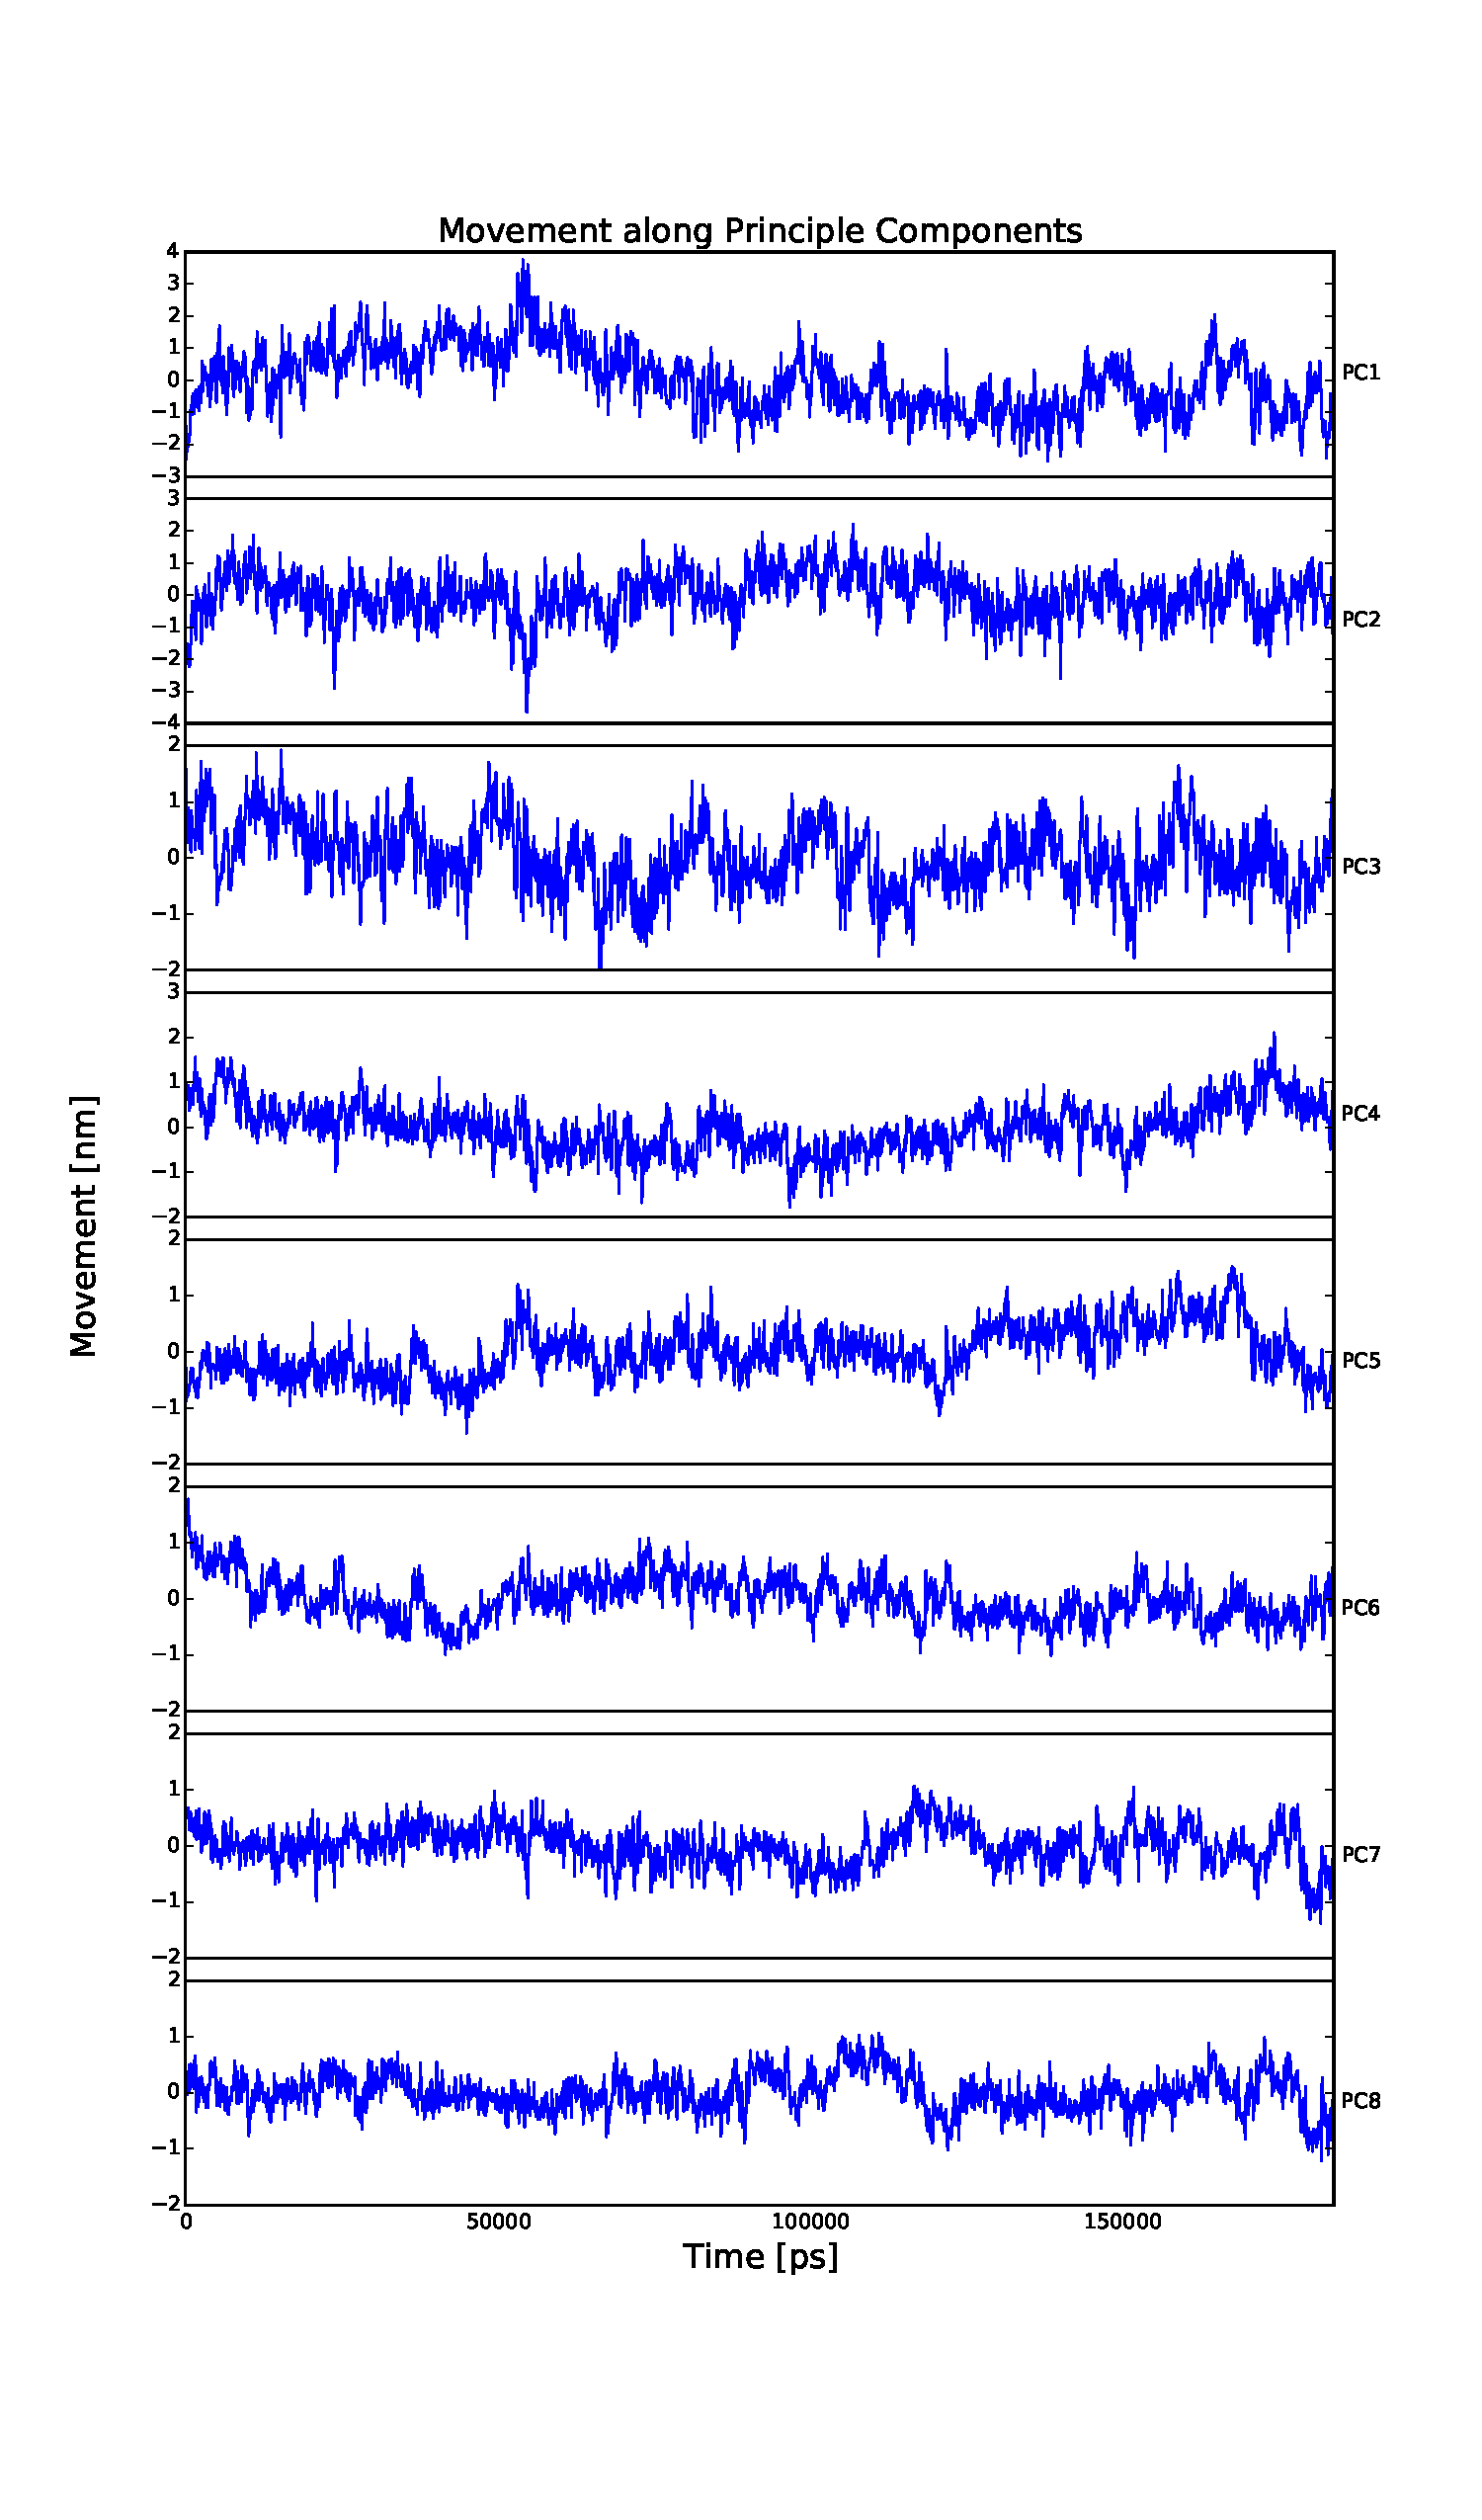
\includegraphics[width=0.7\textwidth]{/home/winz3r/Documents/Protokolle/moleculardynamic/pca_val.pdf}\caption{\centering Projektion der Bewegung auf die ersten acht Hauptkomponenten in Abhängigkeit von der Zeit.}\label{fig:pca_comp}
\end{figure}

Einen besonders guten Einblick in die Dynamik des Proteins liefert die Auftragung der ersten Hauptkomponente gegen die zweite. Dadurch wird die Energielandschaft in der sich das Protein bewegt angedeutet. In Abb. \ref{fig:phasespace1}) wird die Bewegung des simulierten Lysozyms auf die Ebene, die von den ersten beiden Hauptkomponenten aufgespannt wird, projiziert.
\\ \noindent
Da die PCA nicht von der zeitlichen Reihenfolge der Atompositionen abhängt, kann die Simulation des Lysozyms mit experimentell bestimmten Werten verglichen werden.
Dazu wird für eine Reihe experimenteller Strukturanalysen des Lysozyms eine PCA durchgeführt.
In Abb. \ref{fig:exp}) sieht man drei Simulationen mit unterschiedlichen Anfangsstrukturen auf die ersten beiden Hauptkomponenten der experimentellen Daten projiziert.
Deutlich wird, dass Simulation 1 und 2 sich nur in lokalen Minima bewegen, während Simulation 3 die Energiebarriere der beiden Cluster überwindet und sich in beiden Minima bewegt.
Die experimentellen Daten lassen diese lokalen Minima nur erahnen machen aber deutlich, dass die ersten beiden Simulationen nicht genügend Informationen zur Beschreibung der Dynamik des Proteins liefern.

\begin{figure}
\centering
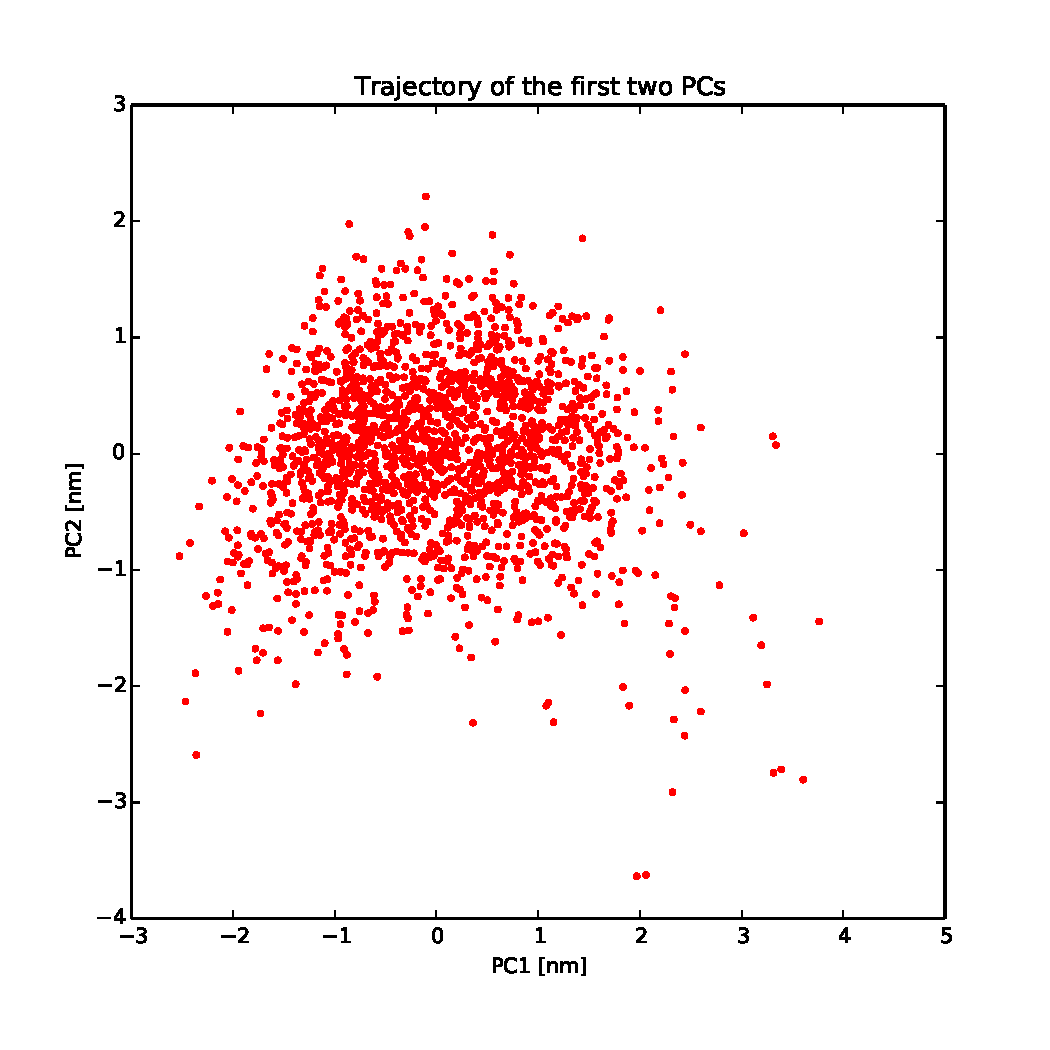
\includegraphics[width=0.7\textwidth]{/home/winz3r/Documents/Protokolle/moleculardynamic/phasespace1.pdf}\caption{Projektion der Bewegung des T4-Phagen Lysozyms auf die ersten beiden Hauptkomponenten. Es wird ein zentraler Cluster der Bewegung deutlich.}\label{fig:phasespace1}
\end{figure}

\begin{figure}
\centering
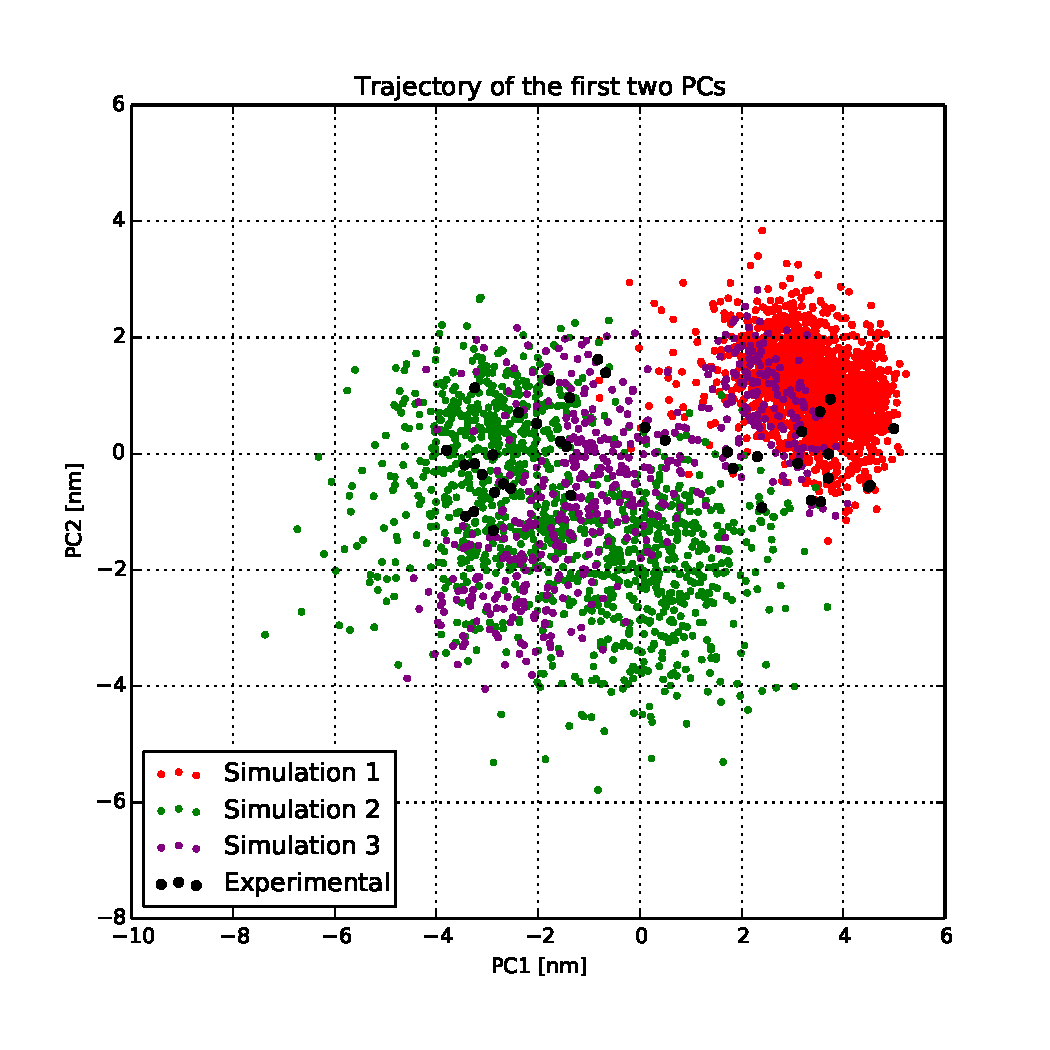
\includegraphics[width=0.7\textwidth]{/home/winz3r/Documents/Protokolle/moleculardynamic/phasespace2.pdf}\caption{Vergleich der aufgezeichneten Bewegung des Lysozyms mit experimentellen Daten. Die Hauptkomponenten sind Resultate der PCA der experimentellen Daten. Es wird deutlich, dass Simulation 1 und 2 nicht den gesamten Raum der möglichen Bewegungen aufzeigen.}\label{fig:exp}
\end{figure}
